\documentclass[fleqn,10pt]{wlscirep}
\usepackage{gensymb}
\title{Impact of Antecedent Land State on Post Landfall Tropical Cyclone Sustenance}

\author[1]{Subashini Subramanian}
\author[2]{Sundararaman Gopalakrishnan}
\author[3]{Robert E. Tuleya}
\author[1,4,*]{Dev Niyogi}
\affil[1]{Purdue University, Department of Earth, Atmospheric and Planetary Sciences, West Lafayette, 47907, USA}
\affil[2]{NOAA/AOML, Hurricane Research Division, Miami, 33149, USA}
\affil[3]{Old Dominion University, Center of Coastal Physical Oceanography, Norfolk, 23508, USA}
\affil[4]{Purdue University, Department of Agronomy – Crops, Soils, Environmental Sciences, West Lafayette, 47907, USA}

\affil[*]{climate.purdue.edu}

%\keywords{Keyword1, Keyword2, Keyword3}

\begin{abstract}
Lack of significant latent heat transfer into the hurricane boundary layer is cited as the typical cause of cyclone post-landfall decay. In this study, the impact of warm and wet land surfaces on tropical cyclone post-landfall evolution is investigated using an idealized version of the Hurricane Weather Research and Forecast (HWRFX2013) model. Results indicate that warmer surfaces are necessary to sustain a storm over land and a wet land surface enhances sustenance. These findings were further analyzed using a quasi-operational, non-idealized modeling study of tropical storm Erin (2007) that intensified post landfall. Results help clarify that the sensible heat flux and resulting enthalpy can be more important than latent heat flux and wet land surfaces alone in terms of causing an environment favorable for post landfall storm sustenance. 
\end{abstract}
\begin{document}
\maketitle

\section*{Introduction}

While the majority of tropical cyclones (TC) decay rapidly post landfall, there are cyclones that have maintained intensity or even re-intensified inland. Recent examples of post landfall sustenance include Tropical Storm (TS) Erin (2007) and TS Fay (2008) in the Atlantic basin, TC Abigail (2001) in Northern Australia, and TC Phet (2010) over the Indian Monsoon Region. The availability of antecedent wet conditions and surface latent heat flux has been thought to be the primary signatures for post-landfall TC intensification\cite{Chang2009PossibleDepressions,Anderson2013}. Re-intensification of TS Erin (2007) over the U.S. Southern Great Plains was analyzed and it was concluded that anomalously wet land conditions can help sustain the storm inland\cite{Evans2011,kellner2012}. Similarly, it has been observed that monsoon depressions respond to high antecedent soil moisture (SM) conditions and their intensity was maintained for a longer duration\cite{Chang2009PossibleDepressions,kishtawal2013}. Thus, a growing number of studies highlight the role of anomalously wet land surface conditions aiding TC sustenance over land.

An outstanding question remains within the literature regarding whether the soil wetness or soil temperature (ST) contributes to post-landfall evolution. For example, Tuleya\cite{Tuleya1994} highlights the influence of soil thermal properties and particularly ST on storm sustenance. Emanuel et al.\cite{Emanuel2008} studied TC Abigail (2001) that re-intensified twice after landfall in Northern Australia in a warm and sandy (high thermal diffusivity) region and concluded that the surface characteristics played an important role in intensifying the storm inland. Kishtawal et al.\cite{kishtawal2012} in their climatological study of TCs over the North Atlantic region also established a positive correlation between post-landfall hurricane intensity and thermal heat capacity of soils. These studies seem to indicate that warm land ST and hence sensible heat flux (SHF) may play a larger role in determining the fate of a storm post landfall. However, an earlier study by Shen et al.\cite{shen2002} concluded that the post landfall decay rate depends on the water content over land as well as, on the surface cooling that controls the potential evaporation. Thus the chief motivation for this study is to contribute to the debate on the relative role of antecedent wet and warm land surfaces on TC post-landfall evolution.

Post-landfall impacts such as flooding from hurricane Sandy (2012) over New York in addition to parallel improvements in land surface models (LSM) and hurricane models such as the Hurricane Weather Research and Forecasting (HWRF) model, are providing momentum for the study of the effects of land surface on TC post-landfall characteristics. As stated, there is still limited understanding of what contributes to the decay, re-intensification or sustenance of a TC over land. Additionally, land feedbacks are at multiple scales (i.e., local boundary layer energetics to mesoscale convergence due to gradients in surface fluxes) and involve multiple parameters as well as processes. In this study, utilizing the realistic processes simulated by the ideal HWRF, we seek to understand the role of land surface characteristics on post-landfall storm evolution. Building off prior studies, the hypothesis that under favorable synoptic settings, a warm land surface is a necessary condition to aid post landfall TC sustenance or re-intensification will be tested. The synergetic relationship between warm and wet soils is also studied.

\section*{Results and Analysis}

The results are presented in two contexts – first for the impact of ST on post-landfall TC evolution using idealized HWRF framework; and then for ST and SM interactions from Factor Separation\cite{SteinnAlpert1993} (FacSep) analysis using both idealized framework and a real case analysis of TS Erin (2007). The model results are analyzed using a number of typical dynamic and thermodynamic features that are typically used for tropical cyclone intensity analysis\cite{Gopal2013,Halliwell2015}. The Hovmöller diagrams are used summarize the fields (winds, surface fluxes, rainfall) with radial distance on the abscissa and the simulation time on the ordinate (e.g. Figure\ref{fig:hove_temp}). The Hovmöller of axisymmetric mean tangential winds is used as the measure of intensity and the discussion is complemented by time series plots of minimum mean sea level pressure (MSLP) and 10 m maximum wind speeds (Vmax).

\subsection*{Soil Temperature Impacts}

To investigate the impact of land surface temperature on TC intensity, a sensitivity study was undertaken by varying the surface temperature from 300 K to 314 K and experiments are named accordingly. The Hovmöller diagram of intensity evolution is presented in Figure \ref{fig:hove_temp} and Supplementary Figure S1 for time series plots of central pressure and winds. In all the experiments, steady state (maximum tangential wind speed is approximately constant) was achieved after around 48 hours from the start of run. A fully mature TC landfall was noted around the 56th hour. For surface temperatures up to 302 K, simulations show a notable drop in intensity immediately after landfall. Similar to Sea Surface Temperature (SST) thresholds for TCs over the ocean (299 – 300 K), 302 K emerged as the threshold ST over land in our simulation. The post-landfall storm evolution remains much stronger when surface temperatures were between 304 and 308 K and re-intensification signatures are noted (i.e., strengthening after initial drop in intensity post landfall). For surface temperatures between 308 and 314 K, sustenance in TC (maintaining landfall intensity) patterns was noted. The wind swaths of cyclones are also significantly larger (45 km for 302 K and 60 km for 308 K after landfall) and enable the storm system to draw in heat and moisture to maintain circulation. Convective precipitation also increased for warmer land surfaces and is shown in Supplementary Figure S2. 

Rainfall has a two primary effects on the soil. While precipitation cools the surface, it also increases the soil heat capacity, neither of which is modeled in HWRF. Rainfall also increases the soil moisture, thus effecting the coefficient of evaporation. Thus, depending on the type of land-surface, the fall in ST may be offset by the higher heat capacity which slows cooling. Note that in the current model configuration, this is simulated by higher surface temperatures for soils with higher thermal diffusivity (cf. Emanuel et al.\cite{Emanuel2008}; Kishtawal et al.\cite{kishtawal2013}). Sandy soil being highly diffusive, supports instantaneous heat transfer which results in higher SHF. The results suggest that storms are stronger when the land is warmer and SHF is higher. Between 80-85\% of the net surface heat flux is comprised of SHF (Figure \ref{fig:hfx_temp}). Through evaporation, precipitation is also recycled back into the storm system increasing latent heat fluxes (LHF) which could further intensify the storm. 

In order to isolate the relative importance of SHF over LHF, an analysis of the total enthalpy fluxes (\(\overline{Q}_E\)) was done next. Halliwell et al.\cite{Halliwell2015} outlined a set of equations to define enthalpy flux (\(\overline{Q}_E\)) for a storm system as
\begin{equation}
\overline{Q}_E(r,t)=\overline{Q}_L(r,t)+\overline{Q}_S(r,t)=\rho_aL_vC_k\bar{v}_{10}(r,t)\Delta\bar{q}(r,t)+\rho_ac_pC_k\bar{v}_{10}(r,t)\Delta\bar{T}(r,t)
\end{equation}
\(\overline{Q}_L\) and \(\overline{Q}_S\) are the azimuthally averaged latent heat and the sensible heat flux components. \(\Delta\bar{q}=\bar{q}_{S}-\bar{q}_{10}\), where \(\bar{q}_{S}\) is the is the surface specific humidity and \(\bar{q}_{10}\) is the specific humidity at 10 m, \(\Delta\bar{T}=\bar{T}_S-\bar{T}_{10}\), where \(\bar{T}_{S}\) is the is the surface temperature and \(\bar{T}_{10}\) is the air temperature at 10 m, \(C_k\) is the surface exchange coefficient for heat and moisture, \(L_v\) is the latent heat of vaporization, and \(c_p\)is the specific heat capacity of air. The difference between enthalpy of the system over the ocean and over land can be attributed to changes in \(\Delta\bar{T}\),\(\Delta\bar{q}\) and \(\bar{v}_{10}\). The change in enthalpy, \(\overline{Q}_E(r,t) - \overline{Q}_E(r,56)\) is expressed as
\begin{equation}
\delta\overline{Q}_E\approx\rho_aL_vC_k\bar{v}_{10}(r,t)\delta\Delta\bar{q}(r,t)+\rho_ac_pC_k\bar{v}_{10}(r,t)\delta\Delta\bar{T}(r,t)+\rho_aL_vC_k\Delta\bar{q}(r,t)\delta\bar{v}_{10}(r,t)+\rho_ac_pC_k\Delta\bar{T}(r,t)\delta\bar{v}_{10}(r,t)
\end{equation}
The reference enthalpy was calculated at landfall (t=56 hours). The sum of first two terms is referred to as the 'land-air part' and the sum of the other two terms is termed the 'wind part'. The enthalpy analysis results are presented as Hovmöller diagrams in Figure \ref{fig:enthalpy}. The difference in enthalpy is negative indicating that the storm is always more intense over the ocean as compared to land. Thus, when the relative difference in the enthalpy is smaller, the post-landfall storm is stronger. The changes in wind speed (\(\delta{v}_{10}\)) and specific humidity (\(\delta\Delta{q}\)) are negative but the temperature difference between land and sea (\(\delta\Delta{T}\)) is positive. Thus, the 'wind part' of the enthalpy contributes to a spinning down of the storm and the thermodynamic part consisting of the \(\delta\Delta{T}\) term (part of the sensible heat component) aids in strengthening the storm. For surface temperatures up to 302 K, the difference in enthalpy for the storm decreases with time. This is because at relatively lower temperatures, the storm decays immediately post landfall and the enthalpy approaches zero which is indicative of storm dissipation. For warmer land, \(\delta\Delta{T}\) is positive compared to cooler land surfaces and the relative difference in \(\delta\overline{Q}_E\) reduces thus increasing the total enthalpy of the system. Difference \(\overline{Q}_E\) in  is almost constant at warmer surface temperatures suggesting sustenance of landfall intensity.
This analysis suggests that warmer land drives higher SHF to increase enthalpy fluxes of the storm ultimately enabling sustenance. These results show that warm soils affect post-landfall storm evolution suggesting that the moisture cutoff after landfall may not be the only reason for post-landfall sustenance of a TC system. The questions then arise, regarding the necessary surface conditions and what surface condition is optimal for storm sustenance. To answer these questions, additional analysis was conducted to isolate the effect of wet and warm soils on post-landfall TCs.

\subsection*{Soil Temperature - Soil Moisture Interactions}

Four representative simulations were analyzed (Table \ref{tab:exp_list}) using a control run (F$_{0}$), one with warmer soil surfaces (F$_{1}$), another with wetter land (F$_{2}$), and a run with both warmer and wetter land (F$_{12}$). This experimental setup or Factor Separation Analysis\cite{SteinnAlpert1993} (FacSep) is used to extract post-landfall intensity changes occurring with an increase in ST from 308 K to 314 K (f$_{1}$), and an increase in SM by 50\% (f$_{2}$) as well as the contribution from both higher ST and SM (f$_{12}$), discussed previously. 

Figure \ref{fig:facsep_ideal} shows the fields of f$_{0}$, f$_{1}$, f$_{2}$, and f$_{12}$ as calculated from the equations outlined in Table \ref{tab:facsep}. It is evident that increasing both SM and ST enhances post-landfall TC intensity. However, the impact of warmer soil is observed almost immediately after landfall whereas the effect of an increase in SM is noted almost 15 hours later. The delayed response of a TC to an increase in SM is consistent with other studies\cite{kellner2012,Evans2011,Chang2009PossibleDepressions} noting the positive impact of antecedent SM conditions on TCs. The f$_{1}$ panel in Figure \ref{fig:facsep_ideal} also shows that the ST effect is relatively high compared to the SM impact on TC intensity. These results suggest that high ST is a dominant and necessary condition for TC sustenance over bare and sandy land. Results for the f$_{12}$ field suggest that not only warm and wet surfaces favor TC sustenance over land, there also exists a synergism where the effect of the combination of the two factors is greater than the individual factors alone. 

To further analyze and verify the above results, a similar FacSep analysis was conducted for a real TC case. TS Erin (2007) was chosen for its distinct strengthening and formation of a post-landfall eye early on 19 August 2007 over Oklahoma. Four experiments were performed using the operational HWRF (v3.7) similar to the idealized FacSep experiments with ST and SM. The experiments were initialized for the 1600 UTC cycle. The physics options are also similar. For the FacSep analysis, the SM and surface temperatures needed to be modified. This was done by increasing the initial fields from National Centers for Environmental Prediction’s Final (FNL) Operational Global Analysis dataset by 50\% for SM and by 6 K for ST for the four layer Noah land surface model that prognostically predicts both ST and SM. These chosen values are guided by multiple idealized sensitivity experiments conducted that show clean signature of both SM and ST. This will enable the model to capture diurnal soil temperature variations as well as surface cooling and soil moisture changes caused by precipitation. The tracks simulated by these experiments are given in Supplementary Figure S3. Due to the relative coarse resolution of the FNL data used to initialize the model, there are significant track errors and the tracks of all experiments consistently show a clear westward bias compared to the observed best track data for TS ERIN. The track errors do not however invalidate the land surface effects observed by the storm mainly because of the large swath of land region that the storm encounters. The results are presented as time series plots for MSLP and Vmax (Figure \ref{fig:facsep_erin}) for F$_{0r}$, F$_{1r}$, F$_{2r}$ and, F$_{12r}$. The results obtained are similar to those from the idealized runs from the previous section. While the experiments capture the broad features well there are notable difficulties in capturing the observed intensity changes, and experiments F$_{1r}$ and F$_{12r}$ shows nominal over land intensification after 84 hours of simulation. Improving the simulation of post landfall characteristics from the HWRF system is an important active research activity and will be a reported in future publications. In the current context, the model does serve its role as a detailed analysis tool to extend the idealized work and study post landfalling systems. When ST was increased initially by 6\degree{C} (F$_{1r}$), the system evolved with lowering of storm central pressure, consistent with the idealized experiments. Increase in SM, in fact, shows increased weakening of storm post landfall compared to observed. F$_{12r}$ shows significant increase in intensity and continues to deepen through 20$^{th}$ of August similar to what was noted in the idealized experiments. The combination of increased soil moisture and soil temperature acts synergistically to setup conditions for post landfall intensification. This result from the TS Erin simulation again highlights that warmer soil emerges as the primary factor supporting re-intensification over land and confirms that the availability of SM helps sustenance. The authors also acknowledge that more detailed analysis of real cases are necessary and study is underway to capture the effect of antecedent land surface conditions in real case scenarios. These results also highlight the importance of accurate representation of the land surface, especially antecedent ST and SM in hurricane models to improve prediction of TC landfall characteristics and warrants attention.

\section*{Conclusion}

This study focused on understanding the effect of land surfaces on post-landfall tropical cyclones. Results indicate that warmer land surfaces support TC sustenance by enhancing system enthalpy. The soil characteristics of the land surface are also critically important to counteract evaporative cooling and increase energy exchange into the boundary layer.  It is evident that under certain conditions for TCs over warm sandy soil, if warm soils can be maintained, and moistened by preceding rains can sustain or re-intensify through rapid transfer of surface heat flux into the atmosphere. 

To investigate the relative importance of ST and SM effects on TC evolution over land, experiments were designed to isolate their impacts and the impact of the interaction between the factors. This was also followed by a real case analysis of TS Erin (2007) using the quasi-operational version of the model. TC response to higher land temperature is relatively rapid as compared to an increase in SM. The magnitude of intensity changes induced by warmer soils is also greater than the intensity changes due to increased soil wetness. This highlights that a warm surface is a necessary condition for TC sustenance post landfall and the SM adds to the increase in energy of the system. A dominant synergism also emerges from the interaction term between these two parameters suggesting that a warm-wet land surface is more favorable for TC sustenance over land than a cold-dry land surface.

\section*{Model Configuration and Experimental Setup}
This study uses the idealized framework of the operationally adopted HWRF (HWRFX2013) with domain settings and physics options (Table \ref{tab:HWRF_phy}) similar to that of Gopalakrishnan et al.\cite{Gopal2013}. The initial cyclonic vortex strength was set to 20 m/s. A typical tropical sounding\cite{Gray1975} was used for temperature and humidity. The HWRFX2013\cite{HWRFdoc2014} system configuration uses the HWRF surface layer parameterization scheme to represent surface layer fluxes and boundary layer processes. In order to individually study the ST and SM feedbacks, the bulk slab land surface parameterization was used for all ideal simulations. 
To simulate landfall, a vortex was introduced and kept fixed at the center of the domain and the land surface was advected at a constant rate. The effect of basic environmental flow and its interaction with the surface is ignored similar to studies by Tuleya and Kurihara\cite{tuleya1978} and Halliwell et al.\cite{Halliwell2015}. The model was integrated for 120 hours with landfall around the 56$^{th}$ hour. An animation of the domain setup is shown in Supplementary Video S1. GFDL land surface model was used for the idealized experiment. It is a single layer land surface model with explicit temperature prediction. This model does not predict soil moisture and is initialized manually. A homogeneous land surface is defined using the model default soil and the vegetation look-up tables and is initialized to dry, bare sandy soil. To extract the feedback processes and interactions in these idealized simulations, land temperature is held constant and diurnal variation effects are eliminated. The model was initialized to the default setting with the following parameters held constant. The ST was set to 308 K and SM at 0.02 m$^{3}$/ m$^{3}$ along with land surface roughness (z$_{0}$) of 0.01 m. The radius of maximum winds that defines the size of the storm was set to 90 km to simulate a moderate-sized storm. To maintain the ocean temperature higher than the threshold value favoring cyclone genesis and evolution, SST was held at a constant 302 K throughout the simulations. A number of experiments were conducted and a subset of 16 experiments was selected to study warm and wet land surfaces as shown in table S2. These experiments seek to isolate the SM and ST impacts on TC evolution following a factor separation (FacSep) approach\cite{SteinnAlpert1993}.  To further evaluate our hypothesis, a real case (TS ERIN (2007)) was run using operational HWRF (HWRF v3.7). The three nested grids were configured with 18:6:2 km. The physics options are the same as in Table \ref{tab:HWRF_phy} (similar to the operational configuration) except Noah land surface model with GFDL surface physics was used to make it as realistic as possible with diurnal and spatial soil moisture, soil temperature evolution.

\bibliography{Mendeley}


\section*{Acknowledgements}

The authors gratefully acknowledge the NSF CAREER – 0847472, NSF R2O (Research to Operations) supplement, Indo-US Science and Technology Foundation (IUSTF) and NOAA’s Hurricane Forecast Improvement Program (HFIP). The authors also wish to acknowledge the Earth System Science Organization, Ministry of Earth Sciences, Government of India (Grant no./ Project no MM/SERP/CNRS/2013/INT-10/002) to conduct this research under Monsoon Mission. The authors also gratefully acknowledge the insights and inputs given by Dr. George Halliwell and thank Dr. Mike Ek, Dr. Vijay Tallapragada and Dr. Joseph Cione for the fruitful discussions and valuable suggestions.

\section*{Author contributions statement}

S.S., S.G., D.N. conceived the experiments, S.S. created a module for the experiments and conducted them. S.S, S.G., D.N. and R.T. were involved in the analysis of experiments. All authors reviewed the manuscript. 

\section*{Additional information}
\textbf{Competing financial interests}
The authors declare no competing financial interests.

%Table 1 -Experimental design
\begin{table}[ht]
\centering
\begin{tabular}{|l|l|}
\hline
\textbf{Variable} & \textbf{Sensitivity Experiments} \\
\hline
Soil Temperature & 300 K, 302 K, 304 K, 306 K, 308 K (default), 310 K, 312 K, 314 K \\
\hline
\multicolumn{2}{c}{\textbf{Factor separation experiments}} \\
\hline
\textbf{Experiment} & \textbf{Factors included (Idealized experiments)}\\
\hline
F$_{0}$ & default run: ST = 308 K, default SM \\
\hline
F$_{1}$ & Soil temperature only; ST=314 K \\
\hline
F$_{2}$ & Soil moisture only; SM+50\% \\
\hline
F$_{12}$ & Soil temperature and soil moisture; ST=314 K and SM+50\% \\
\hline
 & \textbf{Real Case (TS ERIN 2007) Cycle 2007081600 UTC} \\
 \hline
 F$_{0r}$ & Default run \\
 \hline
 F$_{1r}$ & Initial soil temperature increased by 6$\degree{C}$ \\
 \hline
 F$_{2r}$ & Initial soil moisture increased by 50\% throughout the domain \\
 \hline
 F$_{12r}$ & Soil temperature and soil moisture increase \\
 \hline
\end{tabular}
\caption{List of experiments conducted in the idealized HWRF2013}
\label{tab:exp_list}
\end{table}

%Table 2 -FacSep Equations
\begin{table}[ht]
\centering
\begin{tabular}{|l|l|}
\hline
\textbf{Interaction Term} & \textbf{Factor Separation Equation} \\
\hline
f$_{0}$ & F$_{0}$ \\
\hline
f$_{1}$ & F$_{1}$ - F$_{0}$ \\
\hline
f$_{2}$ & F$_{2}$ - F$_{0}$ \\
\hline
f$_{12}$ & F$_{12}$ - (F$_{1}$+F$_{2}$) + F$_{0}$ \\
\hline
\end{tabular}
\caption{Interaction terms and equations for the factor separation analysis}
\label{tab:facsep}
\end{table}

%Table 3 - HWRF physics options
\begin{table}[ht]
\centering
\begin{tabular}{|l|l|}
\hline
\textbf{Physics} & \textbf{Options} \\
\hline
Microphysics & Ferrier Scheme \\
\hline
Cumulus Parameterization & Simplified Arakawa and Schubert (SAS) scheme \\
\hline
Longwave Radiation & GFDL longwave radiation scheme \\
\hline
Shortwave Radiation & GFDL shortwave radiation scheme \\
\hline
Planetary Boundary Layer & GFS PBL scheme \\
\hline
Surface Layer & GFDL surface layer scheme \\
\hline
Land Surface & GFDL slab model, Noah land model (For TS ERIN RUNS)\\
\hline
\end{tabular}
\caption{Physics options used in the idealized HWRF experiments.}
\label{tab:HWRF_phy}
\end{table}

%figure 1
\begin{figure}[ht]
\centering
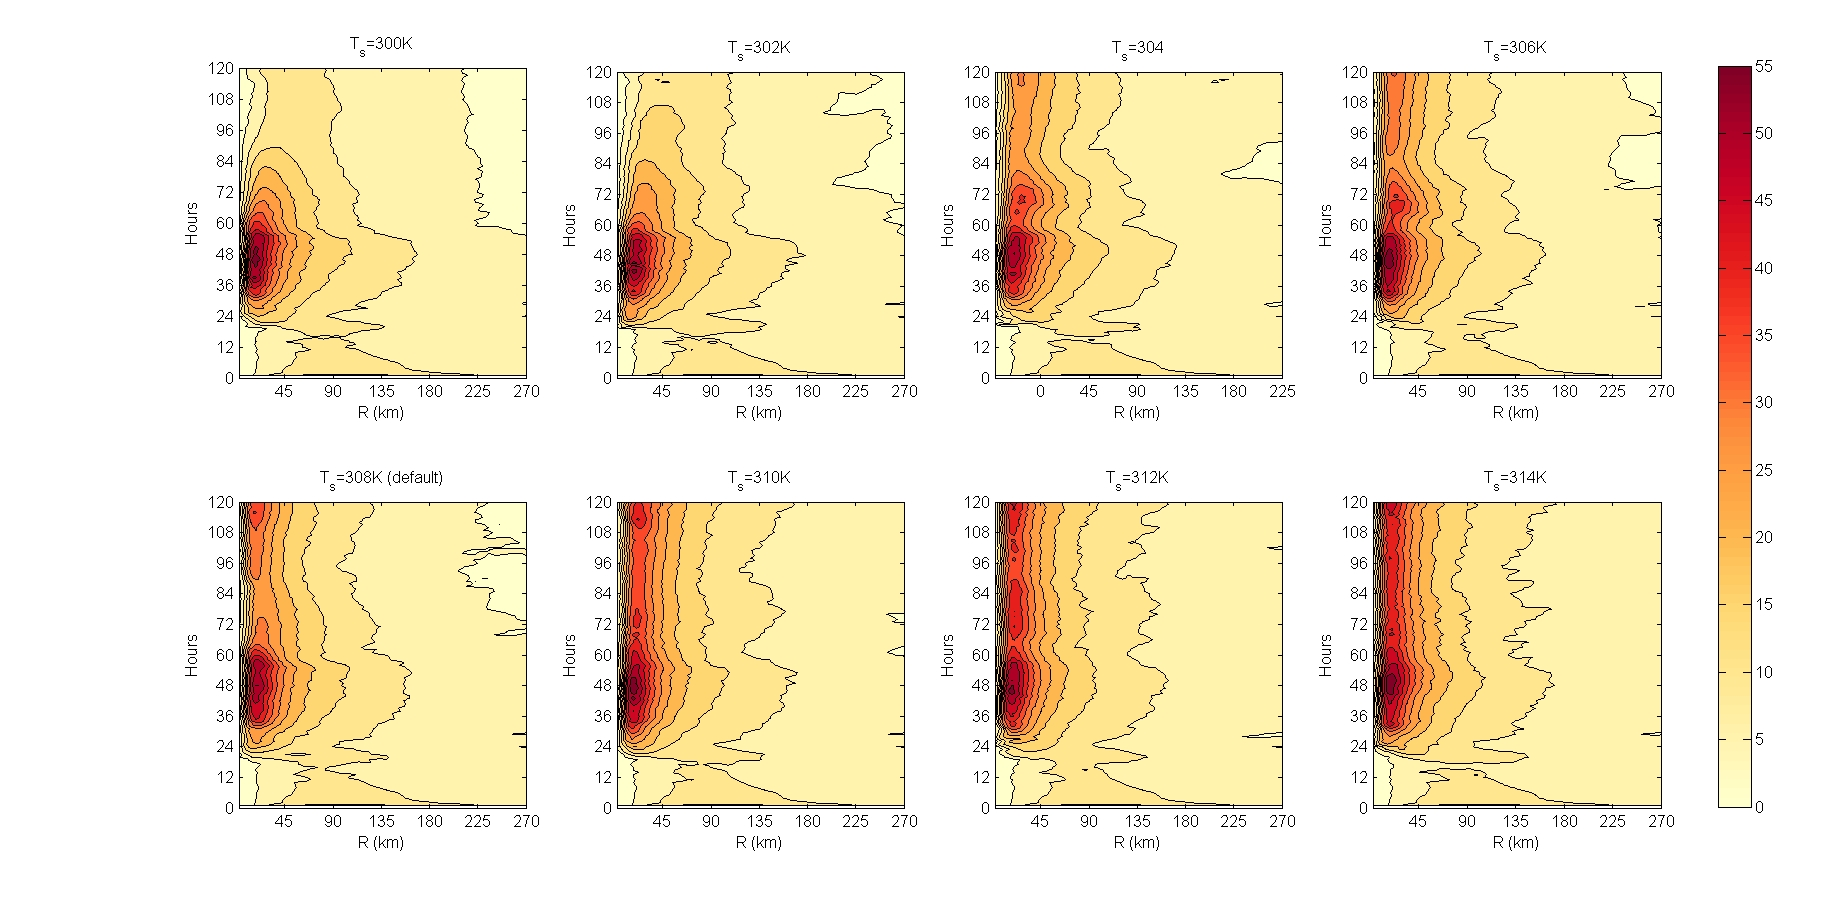
\includegraphics[width=\linewidth]{hove_temp}
\caption{Time evolution (Hovmöller diagram) of azimuthally-averaged axisymmetric 10 m winds (m/s) for different land temperatures (300 K to 314 K). The sea surface temperature was 302 K for all experiments.}
\label{fig:hove_temp}
\end{figure}

%figure 2
\begin{figure}[ht]
\centering
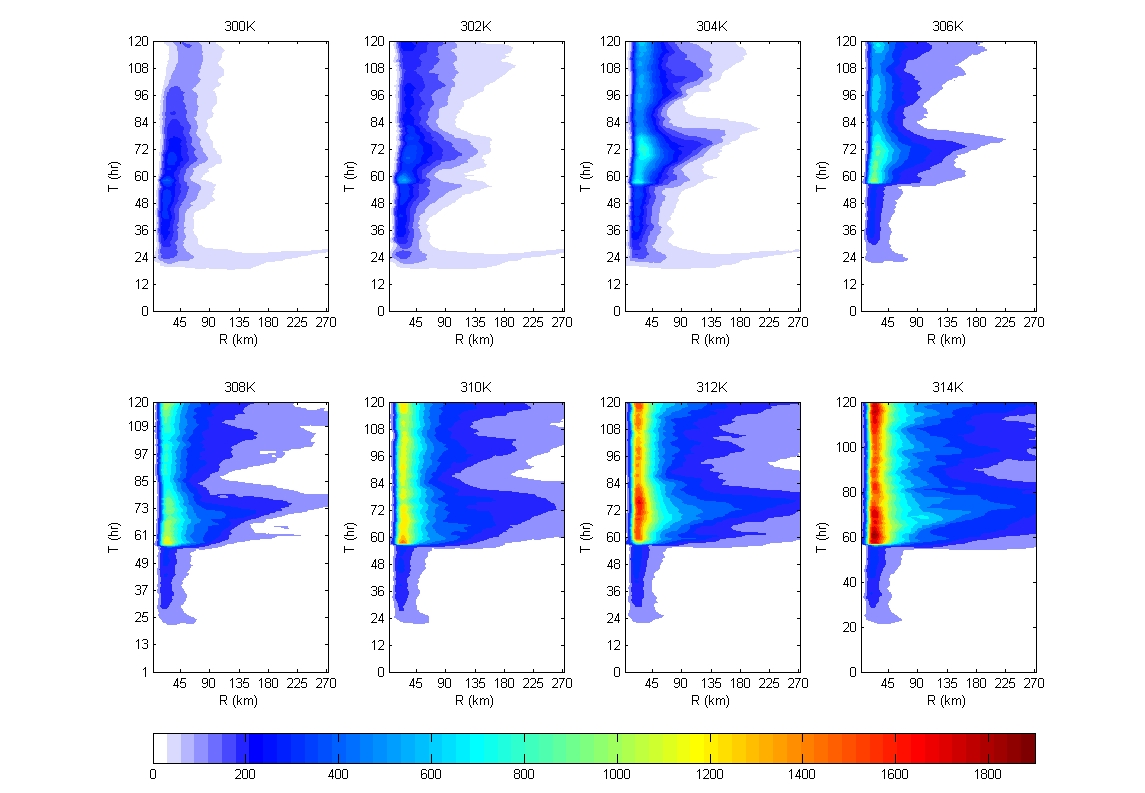
\includegraphics[width=\linewidth]{hfx_temp}
\caption{Hovmöller of sensible heat flux (W/m$^{2}$) corresponding to different soil temperatures (300 K to 314 K).}
\label{fig:hfx_temp}
\end{figure}

%figure 3
\begin{figure}[ht]
\centering
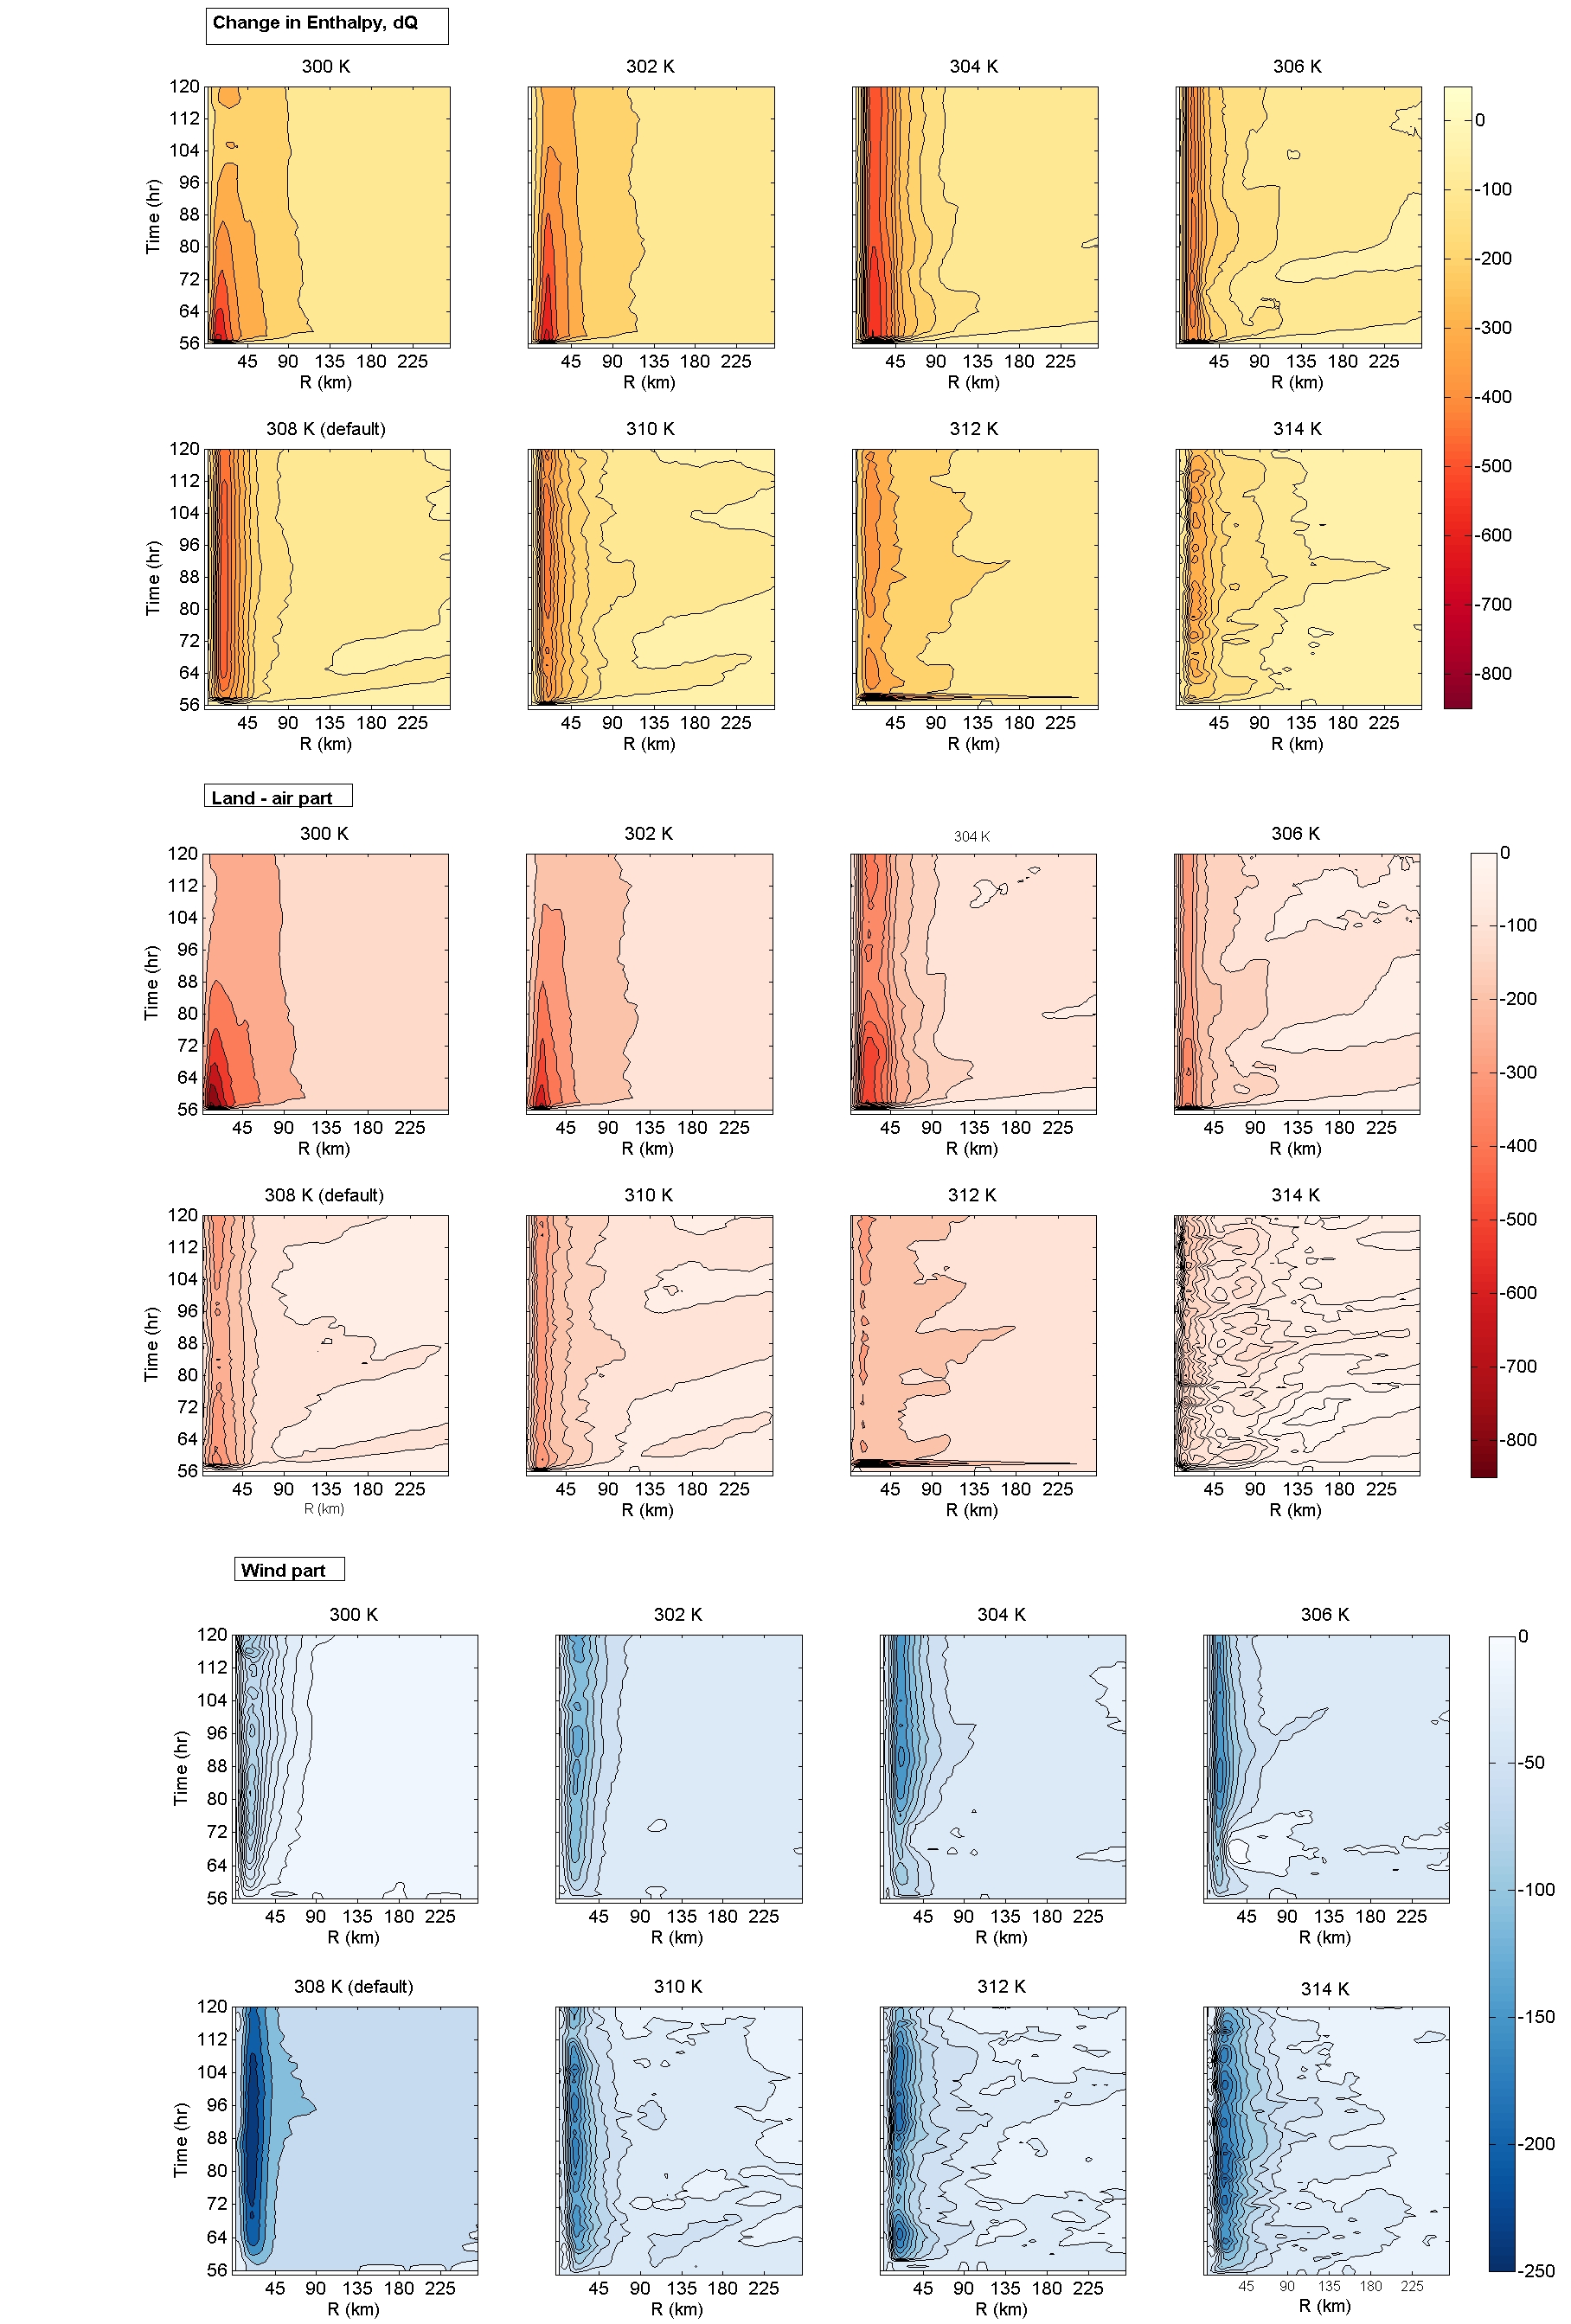
\includegraphics[width=\textwidth, height=\textheight]{dQ_WP_TD}
\caption{Hovmöller diagrams of \(\overline{Q}_E(r,t)-\overline{Q}_E(r,56)\) in W/m$^{2}$ (top panel) and its two primary components from Equation (2): the air-sea part due to changes in  and (middle panel) and the wind part due to changes in wind speed (bottom panel) for different soil temperature experiments.}
\label{fig:enthalpy}
\end{figure}

%figure 4
\begin{figure}[ht]
\centering
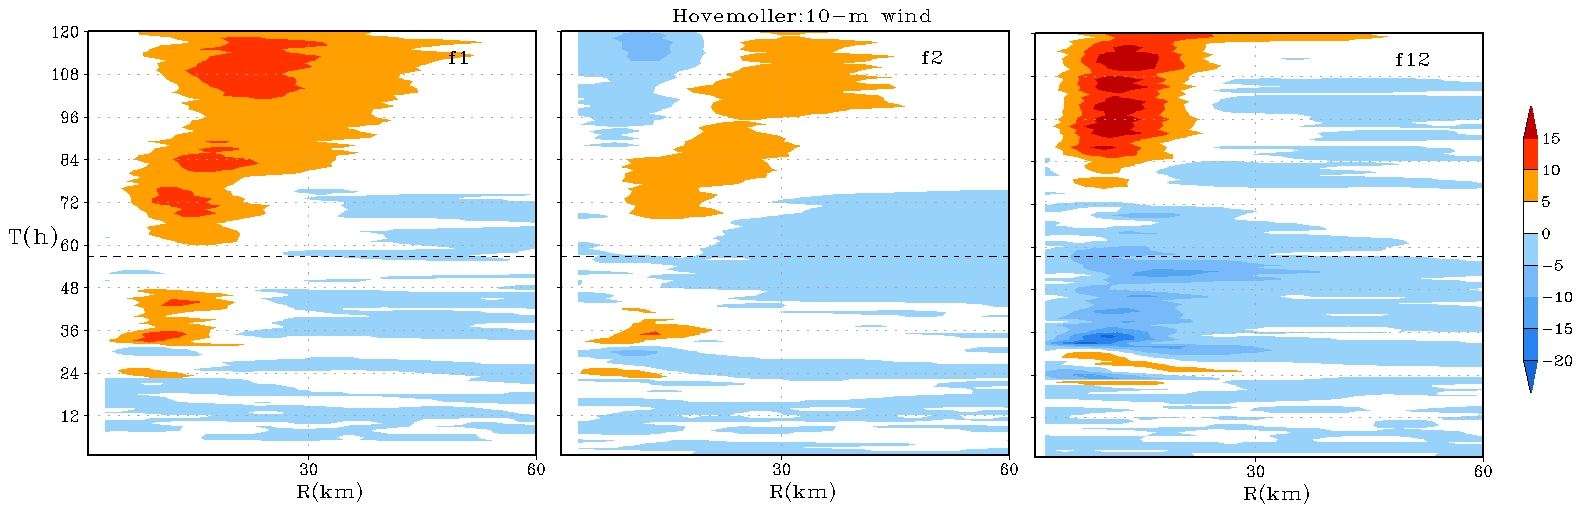
\includegraphics[width=\linewidth]{facsep_mean_winds-2fac}
\caption{Time evolution of mean winds (m/s) around the center of the cyclone to depict the contribution of individual and the interaction of factors in the factor separation analysis.}
\label{fig:facsep_ideal}
\end{figure}

%figure 5
\begin{figure}[ht]
\centering
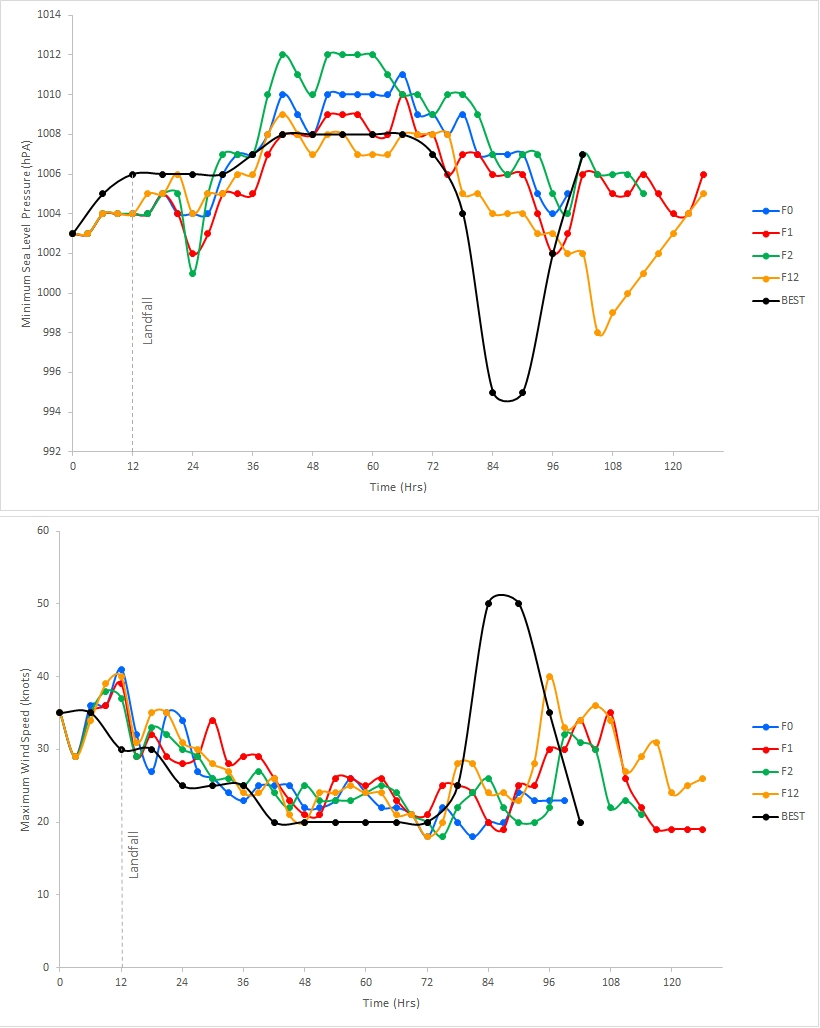
\includegraphics[width=\linewidth]{ERIN_Facsep}
\caption{Minimum sea level pressure (hPa) (top) and maximum sustained 10 m wind speeds in knots (bottom) for TS Erin (2007) in the factor separation experiments}
\label{fig:facsep_erin}
\end{figure}

\end{document}